\documentclass[psfig,preprint]{aastex}
                                                                                
\begin{document}
                                                                                
\title{HOW TO GENERATE MH AND LSFS FILES}

\author{Carl Heiles (\today)}

\tableofcontents


\section{INTRODUCTION} \label{introduction}

	This is basically a cookbook that tells how to perform the first two
stages of GALFA data reduction. If you are interested in details, see
the document entitled ``MH AND LSFS: BLACK-BELT DETAILS''.

	The GALFA spectrometer data are taken every second and are
written in fits files; each fits file usually has 600 seconds worth of
data, with 14 receivers.  We have lots of channels so the files are
large, $\sim 280$ Mbytes.  For further data processing we need to
generate additional files, all of which are much smaller. 

	One of these is the \verb$mh$ file, of which there is one for
every fits file.  The \verb$mh$ file contains two structures called
\verb$mh$ and \verb$mx$.  The structure \verb$mh$ contains accurate
times, positions, and Doppler velocities; the structure \verb$mx$
contains statistical information that can be used to examine whether
the hardware is broken. 

	Another is the \verb$lsfs$ file, which contains the reduced
SMARTF reductions.  The term SMARTF refers to the term used in the
observing GUI to perform Least Squares Frequency Switching (LSFS), so
SMARTF and LSFS are one and the same.  There is one \verb$lsfs$ file for
each SMARTF calibration, and there are usually one or two of these for
each day of observing. 

	One important thing: It is {\it crucial}\footnote{Why is it
crucial? Well, partly because it defines the proper paths to software.
But there's more: the good folks at Goddard changed the conventions in
various routines dealing with time, such as the civil time to LST
converter $ct2lst.pro$, to use east longitude instead of west
longitude. Thus, some of the new Goddard time routines that we use are
not backwards compatible to our software, which uses the old versions.} 
that you start IDL using the
correct startup file. At the very moment (25oct2005), the proper way to do this is
to define the environment variable \verb$IDL_STARTUP$ by typing from the
unix/linux prompt \\
\verb$setenv  IDL_STARTUP ~heiles/gsr/start_ao.idl$ \\
soon we will put the proper file in the \verb$/share/galfa$ area.
Also, you should use a fast
computer such as AOLC1, AOLC2, AOLC3, AOLC4.

\section{GENERATING THE {\it mh} FILES} \label{mhfiles}

	These are used by all analysis routines including the SMARTF
calibration, so these must be generated first. To accomplish this
perform the following steps.

\subsection{Generate the list of fits files} \label{fitsfilegen}

        The first thing to do is generate a file containing a list of
the \verb$fits$ files you are interested in.  You can do this at the UNIX
prompt very easily.  For example, suppose you want all of the \verb$fits$
files for the \verb$togs$ project that reside in a particular
subdirectory (which, at Arecibo, will probably be
\verb$/share/galfa/$). Let's assume the name of this subdirectory is
\verb$togsfilepath$. These \verb$mh$ files have names like
\verb$galfa.20051005.togs.0043.fits$. 

        Get into that subdirectory and type the UNIX command \\
\verb$ls -1 *togs*fits > togsfilelist$ \\
This will produce a file called \verb$togsfilelist$, which will contain
a single column and on each line will be the name of the file (without
any subdirectory prefix). From now on we will refer to this filename
containing the list of fits files as \verb$fitsfilelist$. 

\subsection{Determine the paths for input and output}

	You know the path where the fits files are located; let's call
this fitspath.  In IDL you'd define this variable by \\ 
\verb$fitspath='/share/galfa/'$ \\ 
Also, you've generated \verb$fitsfilelist$.  You need to
know where to {\it write} the \verb$mh$ files you're generating.  Maybe
you want to create a special directory called
\verb$/share/mhname/mymhfiles/$; so in IDL define the path where you'll
put the mh files by \\ 
\verb$mhpath='/share/mhname/mymhfiles/'$

\subsection{The rest is easy\dots}

	You've defined the in and out paths \verb$fitspath$ and
\verb$mhpath$, and the filename containing the list of fitsfiles is
called \verb$fitsfilelist$. You generate all the \verb$mh$ files with \\
\verb$mh_wrap, fitspath, 'fitsfilelist', mhpath$

	There will be several lines of output for each file processed.
Success is indicated by output lines that look like this: \\
\verb$******************writing/share/galfa/galfa.20051005.togs.0003.mh.sav$ \\
The processing time is limited by the speed of reading the fits files,
because they are so large; mostly you'll get
through one file every 3 to 5 seconds. At Arecibo, don't try save clock time by
running two copies of \verb$mhpath$ on the same computer: for unknown
reasons the file-reading time jumps to upwards of 20 seconds!

\section{GENERATING THE {\it lsfs} FILES IN THE STANDARD WAY} \label{lsfsstd}

	Again, the first step is to generate the list of fits files. 
Our software automatically selects groups of SMARTF data from a long
list of fits files that can cover many days.  The easiest way to proceed
is to make a list of all the fits files in your project and let the
program decide what to do.  If you're clever (i.e., lazy) you'll use the
same list of files you used for the \verb$mh$ files above---a list
containing all of the fits files for your project{\footnote{As Kevin
Douglas pointed out, if you're even {\it more} clever you'll know which
fits files contain the LSFS data already, and your list will be much
shorter!}. 

	One thing: every fits file in the list must have a corresponding
\verb$mh$ file.

\subsection{Generate the list of fits files}
	Do this in exactly the same way you did for the \verb$mh$ files,
as described in \S \ref{fitsfilegen}.

	The SMARTF reduction uses the \verb$mh$ files in addition to the
fits files, but you don't need to make a list of \verb$mh$ files because
the program makes it automatically from your list of fits files. 

\subsection{Determine the paths for input and output}

	You need to specify the \verb$fitspath$ and the \verb$mhpath$
for the input files, and also the \verb$lsfspath$ for the lsfs files
that are written.

\subsection{The rest is easy\dots}

	You've defined the in paths \verb$fitspath$ and \verb$mhpath$,
and the output lsfs path \verb$lsfspath$.  You've also defined the
filename containing the list of fitsfiles; let's assume it's the same as
for the \verb$mh$ files, so it's called \verb$fitsfilelist$. 
You generate all the \verb$lsfs$ files with \\ 
\verb$lsfs_wrap, fitspath, mhpath, 'fitsfilelist', lsfspath$ \\
Of course, if you're running IDL in a directory other than the one containing
\verb$fitsfilelist$, then you'll need to specify the path to
\verb$fitsfilelist$. One more thing: the least-squares fit done in the
generation of the \verb$lsfs$ files is a quite complicated iterative
fit, and you can watch it in action by using the \verb$\noquiet$ option:
\verb$lsfs_wrap, fitspath, mhpath, 'fitsfilelist', lsfspath, /noquiet$ \\
This plots the iterative convergence and is fun to watch---for a while,
anyway! 

\section{GENERATING THE {\it lsfs} FILES WHEN THERE ARE PROBLEMS} \label{lsfsprob}

	The standard method might give problems if the \verb$lsfs$ data
were interrupted or restarted, or if the \verb$lsfs$ datataking went
through so many cycles that the resulting data causes a memory overflow.
In either case you need to hand-select the data, and instead of using
the procedure in \S \ref{lsfsstd} you'll need to follow the procedure
below. It involves specifying by hand the specific \verb$fits$ files you
will use and, perhaps, skipping records in the first \verb$fits$ file.
We illustrate with a specific example.

	On 20051120, the \verb$lsfs$ procedure was interrupted and then
restarted. The sequence of l.o.\ frequencies was interrupted and the
automatic selection procedure of \S \ref{lsfsstd} got confused because
the first 277 \verb$lsfs$ records were not applicable to the
\verb$lsfs$ that was actually used. Accordingly, we had to skip over
these 277 records. Moreover, we had to determine that this number was,
indeed, 277---by examining the sequence of l.o.\ frequencies and CAL
state. 

\subsection{Examining the sequence of operations during the $lsfs$
calibration} \label{lsfsex}

\begin{figure}[!p]
\begin{center}
\includegraphics[width=6in]{kevintst0.ps}
\end{center}
\caption{Plots of l.o.\ frequency (top), SMARTF (middle; up means
SMARTF), and CALON (bottom) for the 1200 records in the first two
$mh$ files. \label{kevintst0}}
\end{figure}

\begin{figure}[!p]
\begin{center}
\includegraphics[width=6in]{kevintst1.ps}
\end{center}
\caption{Like figure \ref{kevintst0} but with an expanded horizontal
scale. Plots of l.o.\ frequency (top), SMARTF (middle; up means
SMARTF), and CALON (bottom) for the 1200 records in the first two
$mh$ files. \label{kevintst1}}
\end{figure}

	We begin by performing this examination. The quickest way to do
this is to look at the \verb$mh$ files because they are short and easy
to deal with. We knew beforehand that the first two \verb$mh$ files of
the day contained the \verb$lsfs$ data. Each file is 10 minutes long and
contains 600 records, so we create a 1200-element array of \verb$mh$ structures
so we can plot quantities over the 20-minute interval. Here's the IDL
code we used to make the important plots shown in figure \ref{kevintst0}.

\begin{verbatim}
mhpath= '/dzd5/heiles/togs_1113_to_1115/'       ;where to find the mh files

mhfiles= [ $                                    ;names of mh files to plot
'galfa.20051120.togs.0000.mh.sav', $
'galfa.20051120.togs.0001.mh.sav']

restore, mhpath+mhfiles[0]      ;read the first mh file
mha= replicate( mh[0], 1200)    ;create the 1200 element array of mh structures
mha[0:599]= mh                  ;fill first 600 elements of mha array
restore, mhpath+mhfiles[1]      ;read the second mh file
mha[600:*]= mh                  ;fill second 600 elements of mha array

;NOW DO THE PLOTS...
!p.multi=[0,1,3]
!p.charsize=2
plot, mha.g_lo1/1e6, ytit= 'm1.g_lo1 (LO1 freq, MHz)', /ysty, $
	xtit='Record Nr'
plot, strpos( mha.obsmode, 'SMARTF'), ytit= 'SMARTF?', yra=[-1.1,0.1], /ysty, $
        xtit='Record Nr'
plot, strpos( mha.obs_name, 'ON'), ytit= 'CAL ON',  yra=[-1.1,0.1], /ysty, $
        xtit='Record Nr'
!p.multi=0
!p.charsize=0
\end{verbatim}

	Figure \ref{kevintst0} shows the result. The top panel shows the
l.o.\ frequency versus record number. The initial \verb$lsfs$ data began
near record number 100; the cycle of seven l.o.\ frequencies is clear.
During the second subcycle of this cycle-of-7 the pattern was
interrupted and restarted. The \verb$lsfs$ cycle starts at the lowest
l.o.\ frequency of the set of 7 with SMARTF set on (up in middle plot) 
and has the CAL OFF (down in bottom plot). A single subcycle consists of
a set of 7 frequencies with CAL OFF and a second set with CAL ON.
Normally there are two of these subcycles, so there are 4 7-frequency
sets. In figure \ref{kevintst0}, a set of two subcycles (4 7-frequency
sets) begins at the arrow, which points to record number 277.

	To determine that the record number is 277 instead of, say,
278, we recreate the plots in figure \ref{kevintst0} by limiting the
\verb$xrange$ of the plot (see figure \ref{kevintst1}):

\begin{verbatim}
!p.multi=[0,1,3]
!p.charsize=2
plot, mha.g_lo1/1e6, ytit= 'm1.g_lo1 (LO1 freq, MHz)', yra=[1630,1636], /ysty, $
        xtit='Record Nr', xra=[250,300], /xsty
plot, strpos( mha.obsmode, 'SMARTF'), ytit= 'SMARTF?', yra=[-1.1,0.1], /ysty, $
        xtit='Record Nr', xra=[250,300], /xsty
plot, strpos( mha.obs_name, 'ON'), ytit= 'CAL ON',  yra=[-1.1,0.1], /ysty, $
        xtit='Record Nr', xra=[250,300], /xsty
!p.multi=0
!p.charsize=0
\end{verbatim}

\subsection{Running the $lsfs$ for special cases}

	Given the results from \S \ref{lsfsex}, which consist of the
file names to include and the beginning record number in the first
file, we generate and write the \verb$lsfs$ file with the following set
of IDL commands:

\begin{verbatim}
lsfspath= '/dzd5/heiles/togs_1113_to_1115/'     ;where to write the lsfs file
mhpath= '/dzd5/heiles/togs_1113_to_1115/'       ;where to find the mh files
fitspath= '/dzd5/heiles/togs_1113_to_1115/'     ;where to find the fits files

fitsfiles= [ $                                  ;names of fits files to process
'galfa.20051120.togs.0000.fits', $
'galfa.20051120.togs.0001.fits']

lsfs_shell, mhpath, fitspath, fitsfiles, lsfspath, startndx=277
\end{verbatim}

\noindent {NOTE} that we specify \verb$startndx=277$.  This tells the
program to begin on record number 277 and to ignore records 0 to 276. 
The program reads \verb$mh$ files, deriving their names from the
\verb$fits$ file names, reads the \verb$fits$ files, and automatically
names and writes the \verb$lsfs$ files into the \verb$lsfspath$. 






\acknowledgements This research was supported in part by NSF grant AST 04-06987    
and by the NAIC.

\end{document}
		
